\begin{table}[H]
    {\renewcommand{\arraystretch}{1.2}%
    \setlength{\tabcolsep}{0.3em}%
\begin{tabular}{bababab}
\toprule

\rowcolor{white} \null &
\textbf{Synthetic$_{\mathbf{\mathcal{F}}}$} & \textbf{Synthetic$_{\mathbf{\mathcal{\beta}}}$} &
\textbf{Lehrpfad$_{\mathbf{\mathcal{F}}}$} & \textbf{Lehrpfad$_{\mathbf{\mathcal{\beta}}}$} &
\textbf{Office$_{\mathbf{\mathcal{F}}}$} & \textbf{Office$_{\mathbf{\mathcal{\beta}}}$} \\
\midrule

\rowcolor{lightgray}
\textbf{Keypoint Count} &
    \num{15856} & \num{7851} &
    \num{321529} & \num{243131} &
    \num{30614} & \num{21052} \\
\textbf{Correspondences} &
    \num{6162} & \num{3636} &
    \num{23035} & \num{11428} &
    \num{5288} & \num{2437} \\
\rowcolor{lightgray}
\textbf{True Positives} &
    \num{5997} & \num{3580} &
    \num{18491} & \num{8362} &
    \num{4524} & \num{2119} \\
\textbf{False Positives} &
    \num{4010} & \num{1711} &
    \num{108468} & \num{85075} &
    \num{9348} & \num{7088} \\
\rowcolor{lightgray}
\textbf{False Negatives} &
    \num{165} & \num{56} &
    \num{4544} & \num{3066} &
    \num{764} & \num{318} \\

\bottomrule
\end{tabular}

    }
    \caption[Keypoint and matching results for \texttt{\acrshort{sift}/raw/default}]{\emph{Keypoint and matching results for \texttt{\acrshort{sift}/raw/default}.} The \gls{flexion-image} results in more detected keypoints for all datasets and hence more correspondences. The recall of \acrshort{sift} is outstanding and above 80\% for even the demanding \emph{Lehrpfad} dataset.}
\end{table}
\acrshort{sift} is the most established tested algorithm and therefore evaluated first.
In each dataset the number of detected keypoints and is significantly higher for the \glspl{flexion-image} compared to the \glspl{bearing-angle-image}.
The number of correspondences between keypoints is even approximatly double for \glspl{flexion-image}.
The distribution of the keypoints in each dataset shows no obvious problem in any regard in Figure~\ref{fig:sift_kp_distribution}.
In \emph{Lehrpfad} the keypoints are not as common in the ground area but denser on the walls which is reasonable, as these are the location with most geometry structure.
Similar in \emph{Synthetic}, the rotation of the camera shows a clear trace in the keypoint distribution demonstrating that they stick to geometrically salient regions.
Neither the keypoint sizes, responses or location distribution show surprising characteristics and their distributions are plotted in Appendix~\ref{sec:sift_stats}.

The matching performances most relevant criterion is the descriptors capability to differentiate between salient regions.
For each dataset, except \emph{Synthethic}, the distribution of the descriptor distance of matches shows that true positives and false positives result in a different distribution (Figure~\ref{fig:sift_descriptor_distance}).
Each curve is normalized with the total number of true and false positives per dataset for comparison.
Defining a maximum matching distance threshold will result in less false positives for both conversion types.
The overlapping curves for \emph{Synthethic} are an artifact of the inherent similarity of different regions and can not be avoided.
Appendix~\ref{sec:backprojection_sift} contains plots visualizing the matching performance in each dataset in the actual images.
\begin{figure}[H]
\begin{subfigure}[t]{0.45\linewidth}
    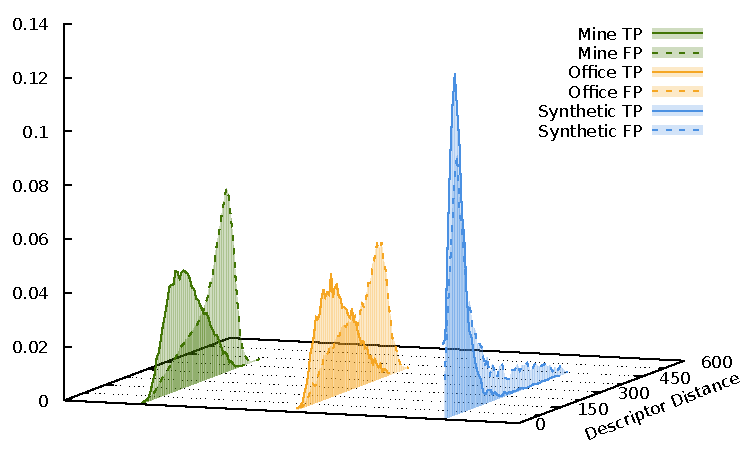
\includegraphics[width=\linewidth]{chapter06/results/SIFT/flexion/descriptor_distances.pdf}%
    \caption{\gls{flexion-image}}
\end{subfigure}\quad
\begin{subfigure}[t]{0.45\linewidth}
    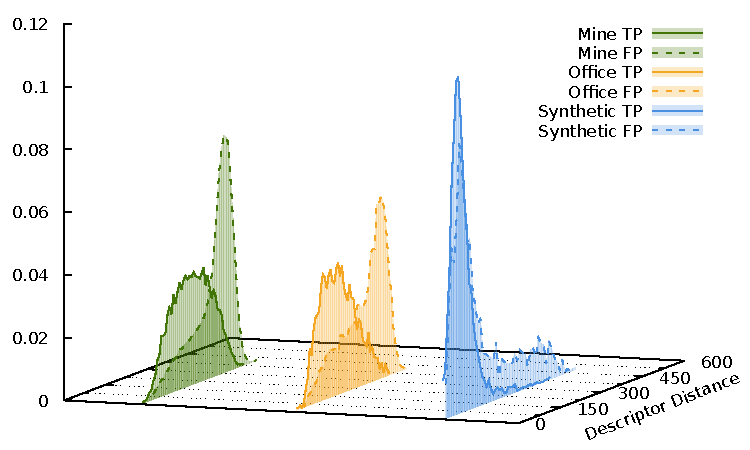
\includegraphics[width=\linewidth]{chapter06/results/SIFT/bearing/descriptor_distances.pdf}%
    \caption{\gls{bearing-angle-image}}
\end{subfigure}
\caption[\acrshort{sift} descriptors distances]{\emph{\acrshort{sift} descriptors distances.} The distributions of descriptor distances show a clear relationship between the distance and the likelihood of a true or false positive. This insight justifies a maximum matching distance to separate false positives better from true positives.}\label{fig:sift_descriptor_distance}
\end{figure}
In terms of the \acrshort{ROC} analysis (Figure~\ref{fig:roc_sift}) the \gls{flexion-image} shows a slightly better performance, but no clear winner can be established.
Additional parameter variation in the \acrshort{sift} algorithm and filtering setup varies the true positive rate by only $5\%$ and the false positive rate by even less.
The differences between the datasets are inherent to their quality and setup.
Most notably, \acrshort{sift} has a very high true positive rate (recall) showing its descriptive power and potential for object recognition tasks.
The very similar false positive rate in all datasets points inherent similarities in the geometries of the scenes that might be explained by the lack of textures as differentiating factor.

Both feature image conversions demonstrate that the salient geometric regions can be recognized with \acrshort{sift}.
The \gls{flexion-image} produces more keypoints and correspondences compared to the \gls{bearing-angle-image}.
Additionally, the true positive rate in \emph{Lehrpfad} is slightly higher in this challenging dataset.
From this the author concludes that the \gls{flexion-image} is better suited.
The theoretical aspects, like rotation invariance and the inclusion of more information per pixel, are additional arguments to prefer the \gls{flexion-image}.
\begin{figure}[H]
\begin{subfigure}[t]{0.45\linewidth}
    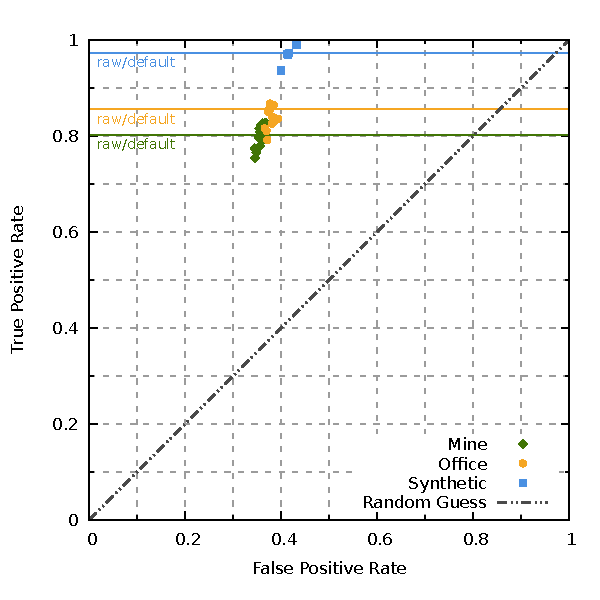
\includegraphics[width=\linewidth]{chapter06/results/SIFT/flexion/roc.pdf}%
    \caption{\gls{flexion-image}}
\end{subfigure}\quad
\begin{subfigure}[t]{0.45\linewidth}
    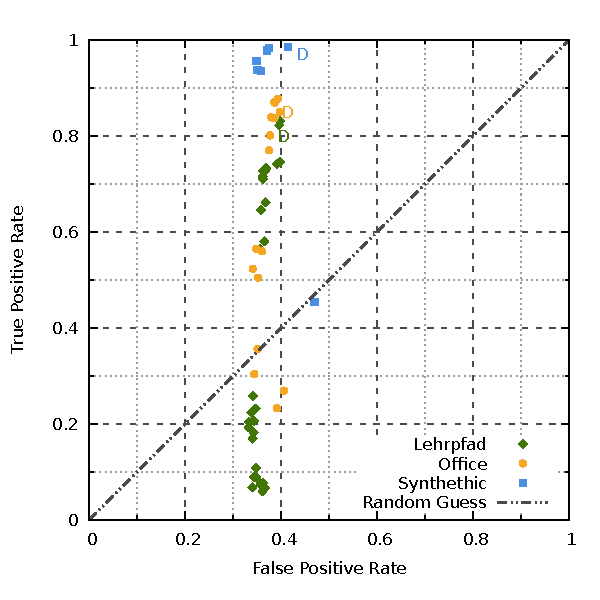
\includegraphics[width=\linewidth]{chapter06/results/SIFT/bearing/roc.pdf}
    \caption{\gls{bearing-angle-image}}
\end{subfigure}
\caption[\acrshort{ROC} graphs for \acrshort{sift}]{\emph{\acrshort{ROC} graphs for \acrshort{sift}.} The \acrshort{ROC} plot for \acrshort{sift} is tightly clustered for both conversions. No distinguished improvements are observable by parameter variations.}\label{fig:roc_sift}
\end{figure}
